% ==========================================================
\section{Feature Model Visualization}
\label{sec:concept_visualization}
% ==========================================================
 
This section defines the visual conventions for representing UVL-based feature models in the proposed editor.
Each decision is motivated using the Physics of Notations~\cite{moody_physics_2009} and, where instructive, contrasted with the conventions established by FeatureIDE~\cite{kastner_featureide_2009}, the de facto reference implementation for feature-model editors.
The goal is to preserve the notation familiarity that domain experts bring from FeatureIDE while making the semantics specific to UVL-BP, namely behavioral elements, root contexts, and rich attributes, directly visible in the diagram.
 
% RQ1

% ----------------------------------------------------------
\subsection{Canonical node structure}
\label{subsec:vis_nodes}
% ----------------------------------------------------------
 
Feature model editors have converged on a labeled-node tree as their canonical representation, and FeatureIDE exemplifies this convention.
A labeled node maps unambiguously to a single feature.
Parent-child edges encode decomposition.
Small decorators at the edge ends encode \textit{mandatory} and \textit{optional} relations.
A set of edges that are part of an \textit{alternative} or \textit{or}-relation is grouped with a distinct circle sector.
This one-symbol-per-construct mapping satisfies \textbf{Semiotic Clarity} and produces a layout that is immediately legible to practitioners trained on any standard notation.
Departing from this topology without a strong semantic justification would violate \textbf{Cognitive Fit}.
Such deviation would also alienate the target audience.
 
The proposed editor therefore retains the node-and-edge structure shown in Figure~\ref{fig:mobile_phone_feature_tree}.
\textbf{Graphic Economy} is maintained by using a single node shape for all ordinary features.
Additional visual channels, such as color, icons, and compartments, are reserved for element types whose semantics genuinely differ from a plain feature.
Overloading the base symbol with decorative variation would reduce \textbf{Perceptual Discriminability}.
It would also unnecessarily inflate the sign inventory.
 
% RQ1

% ----------------------------------------------------------
\subsection{Attribute visibility: UML-style compartments}
\label{subsec:vis_attributes}
% ----------------------------------------------------------

The representation of feature attributes in feature models lacks a unified standard across the literature and tools.
Extended feature models vary widely in their approach: some embed attributes directly within the feature node itself, as shown in Figure~\ref{fig:feature_model_attributes}, while others place attributes in separate external nodes that are then linked to their representative features.
This diversity reflects the absence of consensus on the trade-off between notational economy and semantic transparency.
Each strategy carries distinct cognitive implications for how users perceive the relationship between features and their properties.

\begin{figure}
	\centering
	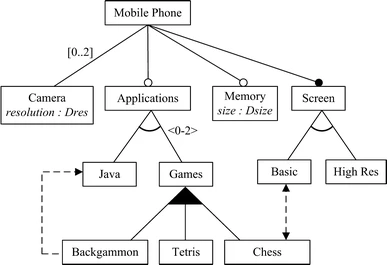
\includegraphics[width=0.6\textwidth]{figures/extended-feature-model-1.png}
	\caption[Feature Model with Attributes]{Example of feature model with attributes. Taken from \cite{karatas_attribute-based_2016}.}
    \label{fig:feature_model_attributes}
\end{figure}
 
FeatureIDE externalizes attributes entirely.
They are accessible only through a separate property view and invisible in the diagram itself.
This can be seen in Figure~\ref{fig:featureide_attributes}.
For a general-purpose feature model, this is a reasonable trade-off in favor of diagram compactness.
For UVL-BP, however, attributes are semantically load-bearing.
They parameterize behavioral definitions and directly influence runtime behavior.
Hiding them behind a panel severs the spatial connection between a feature and its behavioral configuration.
This weakens \textbf{Semantic Transparency} and forces the user to mentally reconcile two disconnected views.

\begin{figure}
	\centering
	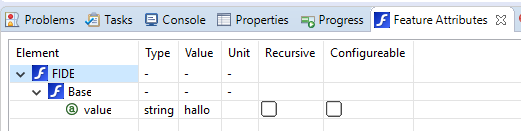
\includegraphics[width=\textwidth]{figures/featureide_attributes.png}
	\caption[Attributes in FeatureIDE]{Feature Attributes View in FeatureIDE. Taken from \cite{bossert_andre_add_2018}.}
    \label{fig:featureide_attributes}
\end{figure}
 
The proposed design adopts a UML-style compartmental node form to address this.
Each node consists of a header row and a lower compartment.
The header row displays the feature name and an optional type glyph, which will be used in the following section.
The lower compartment lists attributes one per line in a compact typeface.
To preserve \textbf{Graphic Economy}, the attribute list is typeset compactly with reduced leading and a smaller font.
Attributes are shown directly in the diagram at all times, except where an attribute is explicitly represented in another form, for example feature-type markers such as \emph{abstract} features.
Attribute lists are not dynamically collapsed or truncated.
The diagram presents them plainly so users can read and act on them without opening secondary controls.
All attribute editing is performed inline in the graphical view through direct-edit affordances.
There is no separate property palette for attribute editing.
The graphical representation therefore serves as the single authoritative editing surface, keeping model structure and attribute values co-located for clear \textbf{Cognitive Integration}.
 
% RQ1 RQ2

% ----------------------------------------------------------
\subsection{Behavioral element types: b-thread and b-event}
\label{subsec:vis_bp-elements}
% ----------------------------------------------------------
 
FeatureIDE's symbol vocabulary already distinguishes certain feature types through visual encoding.
Abstract and concrete features, for instance, employ different color shades and border styles.
This approach satisfies \textbf{Semiotic Clarity} by making semantic differences immediately visible without expanding the node-shape vocabulary.

Felber and Götz present two example visualizations of BP-augmented feature models~\cite{felber_behavioral_2025} (see Figure~\ref{fig:bp-representation}).
In the generic example, b-threads are represented explicitly as blue circles attached to the tree; in the Tic-Tac-Toe example, no separate visual distinction for b-threads is made.
The two images therefore demonstrate that there is not yet a unified semantic convention for representing b-threads in feature trees.
In both examples, b-events are displayed as symbols attached to their parent feature: green circles denote requested events, yellow squares represent waited-for events, and red triangles indicate blocked events.
These event symbols are placed attached to the feature node to show the event-role relationship spatially.

\begin{figure}[ht]
    \centering
    \begin{subfigure}[t]{0.49\textwidth}
        \centering
        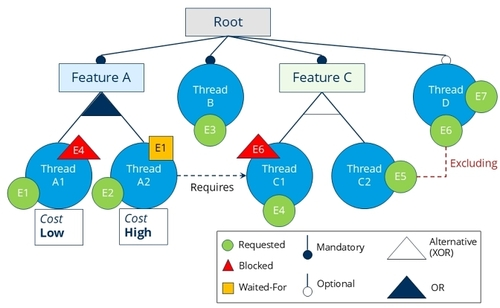
\includegraphics[width=\linewidth]{figures/bp-feature-tree-generic.png}
        \caption{Generic feature tree}
        \label{fig:bp-tree-generic}
    \end{subfigure}
    \hfill
    \begin{subfigure}[t]{0.49\textwidth}
        \centering
        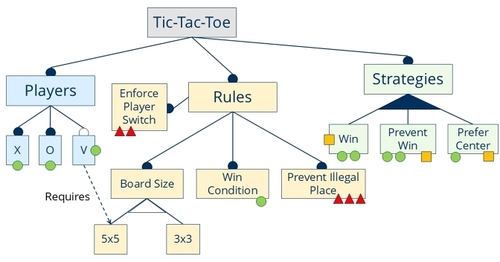
\includegraphics[width=\linewidth]{figures/bp-feature-tree-tic-tac-toe.png}
        \caption{Tic-tac-toe Example}
        \label{fig:bp-tree-tic-tac-toe}
    \end{subfigure}
    \caption[BP examples in feature trees]{Different examples of feature trees with b-threads and b-events. Taken from~\cite{felber_behavioral_2025}.}
    \label{fig:bp-representation}
\end{figure}
 
The proposed tool extends this principle to behavioral elements.
UVL-BP introduces b-threads as a feature with distinct runtime semantics.
It is rendered as a standard compartmental node with an additional type label affixed to the header.
This header decoration clearly marks the behavioral role without introducing a new node shape.
The type reference thus provides \textbf{Perceptual Discriminability} while preserving the familiar node topology.
 
By contrast, a b-event is modeled as a specialized attribute within a feature rather than as a standalone feature node.
Each b-event carries sub-attributes (for example, name and priority) which would be difficult to display if events were represented only as attached symbols on the tree.
Treating events as attributes allows the diagram to show event names and priorities inline in the attribute compartment while still using the distinctive symbols (green circle, yellow square, red triangle) to indicate event type.
This keeps behavioral specifications spatially co-located with their owning feature and preserves \textbf{Semantic Transparency} without sacrificing the expressive detail of event parameters.

To align with the previously described attribute-compartment structure, the proposed tool represents each b-event with a leading icon that encodes its type, followed by the event name and any additional attributes, analogous to the treatment of ordinary attribute entries.
This integration ensures that behavioral specifications are spatially co-located with the feature structure, satisfying \textbf{Semantic Transparency} and avoiding the cognitive dissonance that would result from employing a radically different notation style for behavioral specifications.

\begin{figure}
    \centering
    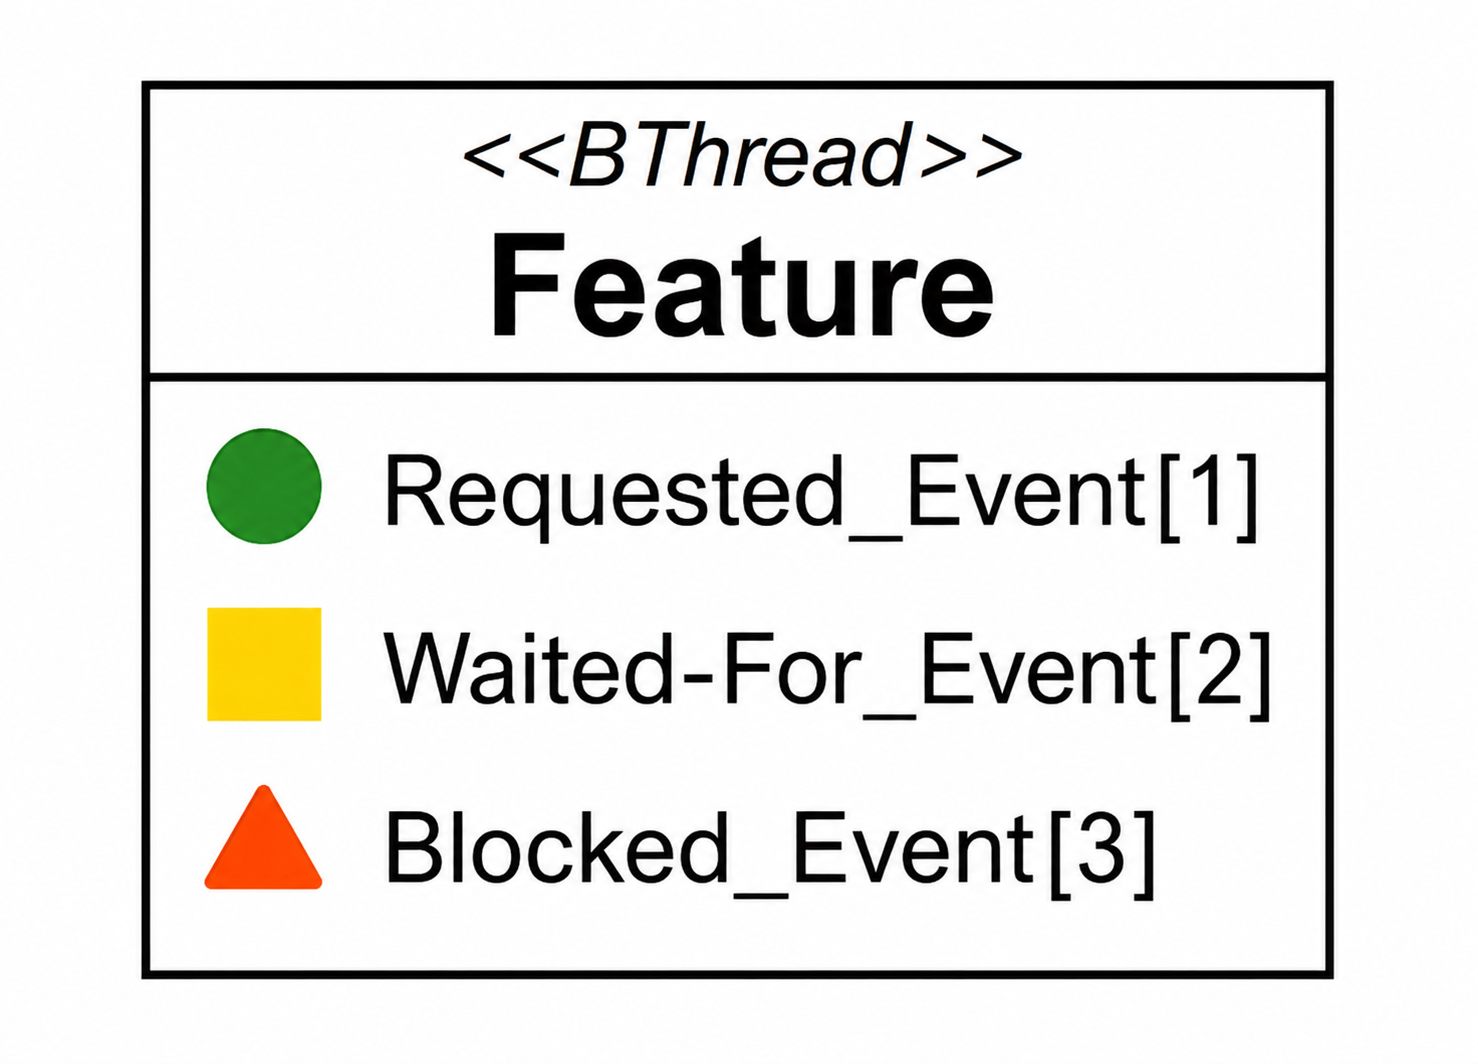
\includegraphics[width=0.6\textwidth]{figures/b_thread_concept.png}
    \caption[Concept of b-thread with b-events]{Conceptual depiction of a b-thread with all three b-event types included in the attribute compartment.}
    \label{fig:b_thread_concept}
\end{figure}

% RQ2 RQ3.2

% ----------------------------------------------------------
\subsection{Constraint representation}
\label{subsec:vis_constraints}
% ----------------------------------------------------------
 
FeatureIDE renders cross-tree constraints in a dedicated textual table below the diagram.
This approach provides no spatial cue about which features are involved.
Users must manually cross-reference the table with the tree.
This weakens \textbf{Dual Coding} and increases cognitive overhead for constraint-heavy models.
 
The proposed design introduces a \emph{binary constraint rule} as an explicit design boundary.
Only binary relations ($n = 2$) are mapped to directed diagram edges.
Constraints involving more than two features ($n > 2$) and complex mathematical expressions are offloaded to a supplementary textual list.
This process of \emph{symbolic offloading} keeps diagrammatic complexity bounded.
It retains full expressive power in the textual form.
The split directly applies Dual Coding Theory.
Binary constraints gain an iconic, spatially anchored representation.
Complex constraints retain a compact symbolic form.
The combination of both channels improves comprehension beyond what either representation achieves alone.

Concretely, binary \textit{requires} and \textit{excludes} relations are rendered in the diagram as dashed, directed cross-tree edges.
Each relation involves exactly two identifiable nodes.
Both types appear pervasively across use cases.
Drawing them as edges preserves the spatial connection between dependent features.
This approach avoids the visual entanglement that afflicts dense multi-hop constraint graphs.
This satisfies \textbf{Dual Coding} and \textbf{Perceptual Discriminability}.
Structural dependencies are encoded in the same visual space as the features they constrain.
This ensures \textbf{Semantic Transparency} for the most common relational patterns.
 
All remaining constraints are collected in a floating constraint list.
This list is part of the graphical canvas and can be repositioned freely.
Users who need close cross-reference with the tree can place the panel nearby.
Users who want to focus on tree structure can move it to the periphery.
This arrangement preserves \textbf{Graphic Economy} for the primary tree view.
All constraints remain immediately accessible without leaving the editor.
\textbf{Complexity Management} is achieved through spatial arrangement rather than through hiding.
This avoids the information loss that a purely collapsible panel would introduce.
 
% RQ1 RQ3.2

% ----------------------------------------------------------
\subsection{Root contexts: \texttt{Env} and \texttt{Config}}
\label{subsec:vis_env-config}
% ----------------------------------------------------------
 
Standard UVL assumes a single root feature from which all other features descend.
UVL-BP extends this with two additional top-level elements, \texttt{Env} and \texttt{Config}.
These elements exist outside the main feature tree.
Neither element carries children.
Instead, both hold attributes that represent global context variables.
Specifically, they represent environmental assumptions and configuration defaults.
Constraints and behavioral definitions across the entire model may reference these variables.
 
\texttt{Env} and \texttt{Config} have no parent-child relationships to any feature in the main tree.
Forcing them into the tree layout would misrepresent their semantics and distort the hierarchy.
Their role is analogous to that of the constraint list.
Both represent globally relevant information that supplements the tree without being structurally part of it.
 
The proposed design therefore treats \texttt{Env} and \texttt{Config} consistently with the constraint list.
Both are rendered as floating, repositionable panels on the canvas.
They use the same compartmental node form as ordinary features.
The header row shows the element name and type glyph.
The lower compartment lists attributes.
Users can position them close to the subtrees or constraints that reference their attributes.
Alternatively, users can move them aside when the focus should rest on the main tree.
This consistent treatment satisfies \textbf{Semiotic Clarity} because ancillary, globally scoped artifacts receive the same visual form.
It supports \textbf{Cognitive Integration} by keeping the full model on a single canvas.
No structural layout is imposed that the semantics do not warrant.
At the same time, the distinct type glyphs in each header ensure \textbf{Perceptual Discriminability} between the two contexts.
 
% RQ2 RQ3.2

% ----------------------------------------------------------
\subsection{Runtime visualization and SSE handling}
\label{subsec:vis_runtime_sse}
% ----------------------------------------------------------

This editor visualizes runtime updates emitted by the FMBP runtime as Server-Sent Events (SSE).
SSE payloads are consumed by the editor extension and translated into transient updates on the canvas.
There are two complementary handling strategies for incoming SSEs.

First, context updates are applied to the floating \texttt{Env} feature.
These updates are rendered in the node's attribute compartment and are not persisted back to the source UVL file automatically.
Persistence requires an explicit user action such as invoking a save command.
This non-persistent visual update keeps the runtime state visible while preserving the source-of-truth principle for model files.

Second, behavioral event notifications are mapped to visual highlights.
When the SSE indicates that a b-event was selected, the server maps it to the owning feature and the b-thread feature that handles the event.
The affected b-thread feature node receives a temporary highlight effect triggered by the client to draw the user's attention.
These visual cues are transient and driven by the live event stream so they communicate runtime activity without altering model contents.

% RQ2 RQ3.2

% ----------------------------------------------------------
\subsection{Multi-model views and VS Code integration}
\label{subsec:vis_multi_models}
% ----------------------------------------------------------

The editor leverages Visual Studio Code's multi-pane UI to display multiple models simultaneously.
Formally, VS Code exposes this capability through Editor Groups and the Split Editor command (workbench.action.splitEditor).
Editor Groups allow users to arrange editors into multiple panes and to view several files side-by-side or in a grid.

For example, four independent model canvases can be arranged in a two-by-two grid so that the user inspects multiple models in parallel.
Each canvas instance binds to a single model file and maintains its own runtime overlay state for SSE-driven visualisation.

To guarantee correct event routing in multi-model layouts, SSE messages must include the file path of the affected model.
The extension uses this path to select the Editor Group and editor instance that hosts the corresponding model canvas.
When the active view for that file is visible, transient updates (Env attribute updates, b-event highlights) are applied to that view only.
If the affected file is open in multiple groups, the extension may propagate highlights to all visible instances for consistent feedback.

This VS Code integration thus enables coordinated multi-model inspection while preserving provenance for SSE-driven runtime updates.

% RQ1 RQ3.2